\documentclass[11pt]{article}

\usepackage[utf8]{inputenc}
\usepackage[french]{babel}

% TODO 1. Géométrie
\usepackage[a4paper,margin=1in,portrait]{geometry}

\usepackage[table]{xcolor}
\definecolor{lightgray}{gray}{0.85}
\definecolor{verylightgray}{gray}{0.95}
\let\oldtabular\tabular
\let\endoldtabular\endtabular
\renewenvironment{tabular}{\small\rowcolors{1}{lightgray}{verylightgray}\oldtabular}{\endoldtabular}

% Pour le bas de page
\newcommand{\mysmallgray}[1]{\scriptsize\color{gray}#1}

\usepackage{comment}

%\usepackage{multicol}
%\setlength{\columnsep}{0.5cm}
\usepackage{wrapfig}

\usepackage{textcomp}
% to use \textcopyleft

\usepackage{graphicx}
\graphicspath{{./yed/}{./images/}{./images-scenario01/}}

% TODO 2. Remplir les champs
\newcommand{\mytitle}{Risus MEGA}
\newcommand{\myauthor}{Olivier Rey}
\newcommand{\mysubject}{Jeu de rôles}
\newcommand{\mykeywords}{JDR,TTRPG,RPG,AideDeJeu,orey,méga,MEGA,messagers-galactiques}
\newcommand{\myversion}{1.0}
\newcommand{\mycolor}{violet}

% PDF
\usepackage{hyperref}
\hypersetup{
  a4paper=true,
  pdftitle={\mytitle},
  pdfauthor={\myauthor},
  colorlinks=true,
  linkcolor=blue,
  urlcolor=blue,
  pdfsubject={\mysubject},
  pdfkeywords ={\mykeywords},
  pdfstartview={FitH},
  bookmarksopen={false},
  bookmarksnumbered={true}
}

% TODO 3. Adapter le titre
\usepackage{fancyhdr}
\pagestyle{fancy}
\fancyhead[L]{}
\fancyhead[C]{{\color{\mycolor}\textbf{{\Huge R}{\LARGE ISUS - }{\Huge R}{\LARGE ÈGLES POUR }{\Huge M}{\LARGE ÉGA}}}}
\fancyhead[R]{}

\fancyfoot[L]{\mysmallgray{Version \myversion}}
\fancyfoot[C]{\mysmallgray{\today}}
\fancyfoot[R]{\mysmallgray{Copyleft \href{https://github.com/orey/jdr-risus}{Olivier Rey}}}
\renewcommand{\headrulewidth}{0.4pt}
\renewcommand{\footrulewidth}{0.4pt}

% Enlève l'indentation pour tout le documnt (équivalent de \noindent sur toutes les lignes)
%\setlength\parindent{0pt}

% Sections avec points après les numéros
\usepackage{titlesec}
\titlelabel{\thetitle.\quad}
\titleformat*{\section}{\color{\mycolor}\bfseries\Large}
\titleformat*{\subsection}{\color{\mycolor}\bfseries\large}
\usepackage[dotinlabels]{titletoc}

%\AtBeginDocument{
%  \addtocontents{toc}{\footnotesize}
%  \addtocontents{lof}{\footnotesize}
%}

% Mes macros

\begin{comment}
\newcommand{\mysection}[1]{
\vspace{0.2cm}
\noindent{\color{\mycolor}\large\textbf{#1}}
}

\newcommand{\mysubsection}[1]{
\vspace{0.1cm}
\noindent{\textit{\textbf{#1}}}
}
\end{comment}

\newcommand{\mybox}[1]{\begin{center}
\noindent\fbox{\parbox{0.8\linewidth}{\small\texttt{#1}}}
\end{center}}

%=======================================DOC
\begin{document}

%=============== Title page

\pagestyle{empty}

\begin{center}

\includegraphics[scale=0.30]{logo-risus}

\vspace{1.0cm}


\includegraphics[scale=1.0]{logo-mega-red}

\vfill

\begin{tabular}{ll}
Méga 1 (1984)       & \href{https://archive.org/details/jeux-et-strategie-hs-1}{Méga 1}, l'origine \\
Méga 2 (1986)       & L'indispensable \href{https://archive.org/details/jeux-et-strategie-hs-2}{Méga 2} \\
Méga 3 (1992)       & Ne peut être trouvé qu'en occasion, voir la fiche \href{https://www.legrog.org/jeux/mega/mega-3/mega-iii-fr-47583}{Grog} \\
Méga 4 (2012)       & Superbes encyclopédie et scenarii sur \href{https://www.messagers-galactiques.com}{messagers-galactiques.com} \\
Méga 5 (2018)       & La \href{https://www.legrog.org/jeux/mega/mega-5e-paradigme/mega-5e-paradigme-fr}{fiche} du Grog \\
Risus EN            & \href{https://www.drivethrurpg.com/product/170294/Risus-The-Anything-RPG}{Risus the RPG} \copyright\ Big Dice Games \\
Risus FR            & \href{https://github.com/orey/jdr-risus/blob/main/risus/risus-fr.pdf}{Risus, traduction de Tristan Lhomme} \\
Sites américains    & Nouveau site : \href{https://www.risusrpg.com}{risusrpg.com} \\
                    & Ancien site : \href{https://www.risusiverse.com/}{risuiverse} \\
Ressources Risus FR & \href{https://rouboudou.itch.io/risus}{rouboudou.itch.io/risus} \\
Copyleft            & Version 1.0 -- \textcopyleft\ \href{https://rouboudou.itch.io}{Olivier Rey} 2022 \\
\end{tabular}
\end{center}

\vspace{0.2cm}

%Note : ce supplément utilise principalement des graphiques pour proposer des règles simples et visuelles.

\tableofcontents

%=============== Fin title page
\newpage
\pagestyle{fancy}

%======= mysection
% TODO Création du personnage
\section{Démarrage de l'aventure}

Le major McLambert convoque les PJs pour le briefing antérieur à la mission.

\begin{wrapfigure}{r}{0.4\linewidth}
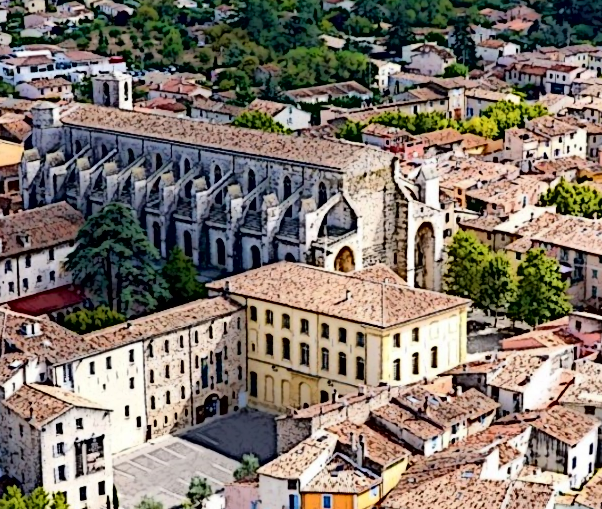
\includegraphics[scale=0.4]{smlsb2}
\end{wrapfigure}

\og{\color{blue}Bonjour. Cette mission doit être menée sur Terre, par des terriens. C'est pourquoi je vous ai fait convoquer.

Comme vous le savez, la Terre est sous surveillance de l'AG, n'étant pas considérée comme assez mûre pour connaître l'existence ni de la Guilde, ni de l'AG. C'est une planète très secondaire, si j'ose dire.

Or, un Guetteur a transmis récemment des informations sur de multiples micro-déchirures de l'InterContinuum dans une petite ville proche d'Aix en Provence, la ville de Saint-Maximin la Sainte Baume. Normalement, les Guetteurs ne s'intéressent pas à ce genre de choses, mais ils ont transmis les informations à un Vieux, Anatole Roublant, dit le Pacha.}\fg


\vspace{0.2cm}

\mybox{Un jeu de \underline{Cliché Méga} réussi avec un \underline{FD = 10} renseignera les PJs sur le fait qu'Anatole Roublant fut un des historiens les plus réputés de la Guilde. Il a dirigé de nombreuses recherches sur l'histoire des univers et est fut un des conservateurs les plus actifs de la grande bibliothèque de la Guilde de ces derniers siècles. On raconte qu'il serait maintenant à la retraire au sanctuaire de Norjane.}

\vspace{0.2cm}

A ce moment, un vieux bonhomme à la barbe blanche entre dans la pièce et enchaîne.

\og {\color{blue}En effet, ces micro-déchirements sont très étranges car ils sont répétés à intervalle régulier et ils semblent liés à des personnes qui passent de manière extrêmement rapide au travers de l'IC, ce qui semble gêner les Guetteurs, comme un genre d'interférences... Nous autres, quand nous transitons,  le voyage n'est pas immédiat. Nous nous guidons à l'emprunte mentale, à l'aide des tétraèdres.

Mais ces personnes ne passent que quelques millièmes de secondes dans l'IC et, elles ne semblent provenir d'aucun point de transit, ni arriver vers aucun. Les Guetteurs sont inquiets, même s'ils ne me disent pas tout.

Votre mission est d'aller sur place, de comprendre le phénomène, de l'arrêter si c'est possible et de revenir au rapport.} \fg

Le Major McLambert donne alors une carte aux PJs avec l'emplacement du point de transit.

\end{document}
